\documentclass[11pt,a4paper]{article}

% === PAQUETES === (((
\usepackage{amsmath}
\usepackage{algorithm2e}
\usepackage{amsfonts}
\usepackage{amssymb}
% \usepackage{expl3}
\usepackage{fontspec}
\usepackage{fullpage}
\usepackage{graphicx}
\usepackage{titlesec} 
\usepackage[shortlabels]{enumitem}
\usepackage{multicol}
% \usepackage{setspace}
\usepackage{dsfont}
\usepackage{xcolor}
\usepackage{url}
\usepackage{listings}
\usepackage{hyperref}
% \usepackage{bookmark}
% )))

% === TIPOGRAFÍA === (((
\setmainfont[
  BoldFont       = bodonibi,
	ItalicFont     = Century modern italic2.ttf,
	BoldItalicFont = bodonibi,
	SmallCapsFont  = lmromancaps10-regular.otf
]{Century_modern.ttf}
% )))

% === COMANDOS === (((
\newcommand{\dis}{\displaystyle}
\newcommand{\qed}{\hspace{0.5cm}\rule{0.16cm}{0.4cm}}
\newcommand{\micita}[1]{\([\)\cite{#1}\(]\)} 
\newcommand{\codigo}[1]{\colorbox{gray!20}{\texttt{#1}}} 
\renewcommand{\_}{\textunderscore}
\newcommand{\operator}[1]{\mathop{\vphantom{\sum}\mathchoice{ \vcenter{\hbox{\huge $#1$}} }
{\vcenter{ \hbox{\Large $#1$}} }{#1}{#1}}\displaylimits}
\newcommand{\suma}{\operator{ 
\includegraphics[scale=0.09]{IMAGENES/Sigma.png}} }
\DeclareSymbolFont{italics}{\encodingdefault}{\rmdefault}{m}{it}
\DeclareSymbolFontAlphabet{\mathit}{italics}
\ExplSyntaxOn
\int_step_inline:nnnn { `A } { 1 } { `Z }
 {  \exp_args:Nf \DeclareMathSymbol{\char_generate:nn{#1}{11}}{\mathalpha}{italics}{#1} }
\int_step_inline:nnnn { `a } { 1 } { `z } {  \exp_args:Nf \DeclareMathSymbol{\char_generate:nn{#1}{11}}{\mathalpha}{italics}{#1}}
\ExplSyntaxOff
% )))

% === SECCIONES === (((
\titleformat*{\section}{\large\normalfont\bfseries}
\titleformat*{\subsection}{\large\itshape \centering}
% \setcounter{secnumdepth}{0}
\setcounter{tocdepth}{2}
\renewcommand*{\contentsname}{\large\textbf{CONTENIDOS.}}
\usepackage[nottoc,numbib]{tocbibind}
\renewcommand{\refname}{REFERENCIAS.}
\renewcommand{\tablename}{Tabla}
\renewcommand{\figurename}{Figura}
% )))

% === PORTADA === (((
% \pagestyle{empty}
\newcommand{\portada}{
\addfontfeature{LetterSpace=-5}
  \begin{titlepage}
  \centering
  \begin{figure}
    \centering
    
\includegraphics[scale=0.5]{IMAGENES/logo_uaa.png}  
  \end{figure}
  {\bfseries\Large\MakeUppercase{\textit{Universidad Autónoma de Aguascalientes.}} \par}
  \vspace{1cm}
  {\Large Centro de Ciencias Básicas. \vspace{0.5cm}\\[2mm]
  Departamento de Estadística.\vspace{0.5cm}\\[2mm]
  Licenciatura en Matemáticas Aplicadas.\vspace{0.5cm}\\[2mm]
  Proyecto 1.\par}
  \vspace{1.5cm}
  {\bfseries\Huge ¿Qué Lenguaje de Programación\\se Ejecuta más Rápido? \par} % title
  \vspace{1.5cm}
  % {\itshape\Large Óptica. \\Prof. Mariana Alfaro Gómez.\par}
  % {\itshape\Large Variable Compleja I. \\Prof. Fausto Arturo Contreras Rosales.\par}
  % {\itshape\Large Métodos Numéricos II. \\Prof. Manuel Ramírez Aranda.\par}
  {\itshape\Large Diseño de Experimentos. \\Prof. Angélica Hernández Quintero.\par}
  % {\itshape\Large Filosofía de la Investigación Científica. \\Prof. Jesús Mariano Rodríguez Muñoz.\par}
  \vfill
  % {\Large \textit{Por Erick I. Rodríguez Juárez.}\par}
		\begin{center}
		\Large
		Alumnos:\\
		\textit{Juan Daniel Medina Jiménez.}\\
		\textit{Erick Ignacio Rodríguez Juárez.}
		\end{center}
  \vfill
		% \begin{flushright}
		% {\Large Realización: <++>\(/\)<++>\(/\)22. \par} % date
		% {\Large Entrega: <++>\(/\)<++>\(/\)22. \par} % date
		% \end{flushright}
		\begin{center}
			\Large Domingo 8 de Mayo, 2022.
		\end{center} 
  \end{titlepage} 
	\thispagestyle{empty}
	% \doublespacing
	\tableofcontents
	% \singlespacing
	\newpage
} 
% )))

% === LSTLISTINGS === (((
\definecolor{backcolour}{rgb}{0.95,0.95,0.92}
\lstdefinestyle{mystyle}{
  backgroundcolor  =  \color{backcolour},
  commentstyle     =  \color{gray},
  numberstyle      =  \tiny\color{gray},
  stringstyle      =  \color{purple},
  basicstyle       =  \ttfamily\footnotesize,
  numbers          =  left,
  numbersep        =  5pt,
  keywordstyle     =  \color{blue},
  identifierstyle  =  \color{purple},
}
\lstset{style=mystyle}
% )))

\begin{document}

\portada

% TODO: REESCRIBIR.

\section{INTRODUCCIÓN.} % (((

\subsection{--- Motivación ---} % (((
\label{sub:motivacion}
El desarrollo de programas computacionales (y la construcción de nuevos lenguajes de programación) ha ofrecido poderosas herramientas y técnicas para la extensión de las profesiones mejorando su productividad.
Con algunas tareas, para continuar con un ascenso en la eficiencia, se requieren crear y desarrollar tecnologías cuyo objetivo principal sea el de producir programas cada vez más rápidos.
Sin embargo, la gran cantidad de lenguajes existentes (cada uno con diferentes implementaciones y funciones únicas) puede hacer que se desvíe la tarea por escribir el programa más eficiente en términos de recursos algoritmicos, y sea reemplazada por la búsqueda de paqueterías y lenguajes que integren las funciones deseadas, y los problemas resueltos.
El enfoque inverso también representa una problemática: si el lenguaje en el que se programa para resolver una determinada tarea es ineficiente en términos de recursos computacionales para la implementación del algoritmo escrito, es conveniente migrar a otro lenguaje que realice tal proceso en una cantidad de tiempo menor.

Estos dos problemas son de interés para dos sectores.
Primero, las empresas que requieran soluciones técnicas y específicas.
Segundo, las personas que realicen investigación individual y el público que necesite implementar funciones para hacer su profesión (y\(/\)o su informática personal) mejor adaptada a sus necesidades.
El presente trabajo está encaminado a resolver ésta problemática para las personas del segundo sector, dado que en una empresa pueden llegarse a obtener mejores recursos computacionales y solucionar su informática por fuerza bruta o algoritmos menos óptimos.

En la lista siguiente (obtenida de \micita{lenguajes_importantes}) se incluyen los lenguajes de programación más conocidos y sencillos, cuyos compiladores (o programas de ejecución) son suficientemente ligeros para instalarse en un ordenador promedio casero.\\
\begin{minipage}{0.33\linewidth}
\begin{enumerate}[noitemsep]
	\item \texttt{C.}
	\item \texttt{Python.}
	\item \texttt{R.}
	\item \texttt{Ruby.}
\end{enumerate}
\end{minipage}\hspace{5mm}
\begin{minipage}{0.33\linewidth}
	\begin{enumerate}[noitemsep]
	\setcounter{enumi}{4}
	\item \texttt{Matlab\(/\)Octave.}
	\item \texttt{Rust.}
	\item \texttt{Java.}
	\item \texttt{Lua.}
	\end{enumerate}
\end{minipage} \hspace{5mm}
\begin{minipage}{0.33\linewidth}
	\begin{enumerate}[noitemsep]
		\item \texttt{C++.}
		\item \texttt{JavaScript.}
		\item \texttt{Golang}
		\item \texttt{Perl.}
	\end{enumerate}
\end{minipage}\\[2mm]
Se seleccionarán para objeto de estudio, los primeros \(4\) lenguajes: \texttt{C}, \texttt{Python}, \texttt{R}, y \texttt{Ruby}, debido a que son de los más conocidos y simples en escritura para funciones del segundo sector demográfico mencionado, consulte \micita{popularidad}.

El objetivo es determinar estadísticamente el tiempo promedio en que una misma secuencia de tareas (algoritmo) se logra ejecutar en cada uno de los lenguajes seleccionados, y medir en cuánto difieren en su tiempo promedio de ejecución.
Para ello, se someterá a todos los programas escritos en los \(4\) lenguajes a seguir el mismo algoritmo, a pesar de que (posiblemente) existan formas más eficientes de lograr la tarea propuesta, ya sea por medio de paqueterías adicionales al lenguaje, o bien, por funciones que se ofrecen de forma nativa.

Se tiene conocimiento del estudio comparativo realizado en \micita{comparacion_lenguajes}, cuyo objetivo es el de observar la cantidad de energía gastada por cada lenguaje.
En tal análisis se realiza la recolección de \(10\) problemas de programación bien conocidos, escritos en \(27\) lenguajes de programación.
No obstante, examinando el código en \micita{github_rosseta}, se observa que se seleccionaron distintos algoritmos con diferentes órdenes de complejidad para resolver la misma tarea en algunos lengujes, tales como en la obtención del \(n-\)ésimo número de Fibonacci en \texttt{C}, y \texttt{Python}.
El presente trabajo pretende exponer ejemplos más sencillos, pero estandarizados para evaluar a los lenguajes de programación expuestos.
% )))

\subsection{--- Diseño de Experimentos ---} % (((
\label{sub:diseño}

\subsubsection{Definición de Diseño Experimental.} % (((
\label{subs:definicion_de}
Un \textit{experimento} es una sucesión de pasos que cambian las condiciones de operación de un sistema.
Su objetivo en el planteamiento es el de determinar el efecto producido por las características variables en el estudio.
Son escogidos un conjunto finito de condiciones a las que serán cometidos unos sujetos (u objetos) determinados para medir la respuesta producida por el cambio de condiciones. \\[2mm]
Éstas con las características de un diseño experimental.
\begin{enumerate}
	\item \textit{Unidad Experimental:} Objeto al que se registrará las mediciones de todo el experimento.
	\item \textit{Variable Respuesta:} Característica medible (con unidades) de la unidad experimental.
	\item \textit{Factores Controlables:} Características del experimento que siempre podrán ser manipulables y que podrán ser manipulables en cualquier otro experimento análogo.
	\item \textit{Niveles de Factor Controlable (tratamientos):} Categorías disponibles del factor controlable (\(T_1, \;\ldots,\; T_k\)).
	\item \textit{Factores de Ruido:} Características del experimento que interfieren con la unidad experimental. No necesariamente son las mismas en otros experimentos análogos.
	\item \textit{Número de Repeticiones por tratamiento:} Número de veces en que se realiza una medición en el mismo nivel de factor controlable, y en los mismos factores de ruido.
	\item \textit{Número de Corridas Experimentales:} Número total de mediciones.
	\item \textit{Balanceo:} Un diseño es balanceado si se realizó el mismo número de mediciones en cada nivel de factor controlable.
\end{enumerate}
En algunos diseños se tiene adicionalmente el siguiente concepto.
\begin{enumerate}
	\setcounter{enumi}{8}
	\item \textit{Factor Bloque:} Factor de ruido que es manipulable en el experimento.
	\item \textit{Niveles de Factor Bloque:} Categorías disponibles del factor bloque (\(B_1, \;\ldots,\; B_n\)).
\end{enumerate}
Se tiene como principio el de determinar el orden de las corridas experimentales de forma \textit{aleatoria}, esto es, que no se tenga elección sobre el orden de presentación de factores de ruido y controlables al momento de realizar la recolección de mediciones.
Consulte \micita{gutierrez}.
% )))

\subsubsection{Definición de un Diseño Cuadro Latino.} % (((
\label{subs:definicion_dcl}
Un \textit{Diseño Cuadro Latino} (DCL) es un diseño experimental lineal con un sólo factor controlable con \(k\) tratamientos (\(T_1, \;\ldots,\; T_k\)), dos factores de bloque, cada uno con \(k\) niveles (\(A_1 , \;\ldots,\; A_k\) y \(B_1, \;\ldots,\; B_k\)), de tal manera que por cada posible configuración de bloque sólo exista un medición de un factor controlable que no se repita en el mismo Bloque 1, o Bloque 2.
Así, la Tabla \ref{tab:cuad_lat_4} es un DCL \(4 \times 4\).
Usualmente los tratamientos se enumeran con las letras \(A,B, \;\ldots\;Z\) y los niveles de bloque se establecen al inicio del experimento, indicando cuál será la fila y cuál la columna.
De modo que la representación final se obtiene en la Tabla \ref{tab:representacion}.
\newpage
\begin{table}[ht!]
	\begin{minipage}{0.5\linewidth}
	\centering
	\begin{tabular}{c|*{4}{c}}
					& \(A_1\) &	\(A_2\) &	\(A_3\) & \(A_4\) \\ \hline
		\(B_1\) & \(T_4\) & \(T_2\) & \(T_3\) & \(T_1\) \\
		\(B_2\) & \(T_2\) & \(T_4\) & \(T_1\) & \(T_3\) \\
		\(B_3\) & \(T_1\) & \(T_3\) & \(T_4\) & \(T_2\) \\
		\(B_4\) & \(T_3\) & \(T_1\) & \(T_2\) & \(T_4\) \\
	\end{tabular}
	\caption{Ejemplo de DCL no--estándar.}
	\label{tab:cuad_lat_4}
	\end{minipage}\hspace{5mm}
	\begin{minipage}{0.5\linewidth}
		\centering
		\begin{tabular}{*{4}{c}}
		D & B & C & A \\
		B & D & A & C \\
		A & C & D & B \\
		C & A & B & D
	\end{tabular}
	\caption{Representación de DCL del la Tabla \ref{tab:cuad_lat_4}.} 
	\label{tab:representacion}
	\end{minipage}
\end{table}
Un DCL es \textit{estándar}, en caso de que  la primer fila conste de los tratamientos ordenados \(T_1, \;\ldots,\; T_k\).
Cualquiera de los DCL puede obtenerse a través de la permutación de filas y columnas de un DCL estándar.
La formulación matemática es la siguiente. Sean
\[
	Y_{ij(h_{ij})} : \Omega \longrightarrow \mathds{R} , \hspace{5mm} Y_{ij(h_{ij})} \sim N(\mu + \tau _{h_{ij}} + \gamma _i +\delta _j, \sigma ^2), \hspace{5mm} i,j \leqslant k.
\]
donde a \(\mu\) se le llama \textit{gran media}, \(\tau _{h_{ij}}\) es el efecto del \(h_{ij}\)--ésimo tratamiento, \(\gamma _i\) es el efecto del \(i\)--ésimo nivel del bloque 1, y \(d_j\) es el efecto del \(j\)--ésimo nivel del bloque 2.
Hay que estimar \(\{\mu , \tau _{h_{ij}} , \gamma _i , \delta _j\}\) y además se asume que
\begin{equation}
	Y_{ij(h_{ij})} = \mu + \tau _{h_{ij}} + \gamma _i+ \delta _j + \varepsilon _{ij(h_{ij})}.
	\label{eq:modelo}
\end{equation}
es decir, \(\varepsilon _{ij(h_{ij})} \sim N(0, \sigma ^2)\), y es una variable aleatoria llamada \textit{residual}.
Para esto, consulte \micita{cox}.
Las preguntas principales a responder en un DCL son las siguientes.
(Se les llama hipótesis porque no se conoce su veracidad y las proposiciones se podrán a prueba de los datos recolectados).
Se le llama \(H_0\) a la \textit{hipótesis nula}, y \(H_a\), \textit{hipótesis alternativa}.
\begin{enumerate}
	\item[\fbox{Hip. Principal}]
		\begin{equation}
			\begin{array}{rl}
				H_0 :& \tau _1 = \;\cdots\; = \tau _k = 0, \\[2mm]
				H_a: &\exists h \;:\; \tau _h \ne 0.
			\end{array}
			\label{eq:hipotesis_principal}
		\end{equation}
		La cual, es probada con el estimador \(F_{trat} = CM_{trat} / CM_E\) de la tabla ANOVA de la sección.
% TODO: COLOCAR SECCIÓN LINEA 139.
		Y \(H_0\) significa que no hay diferencia entre tratamientos.
	\item[\fbox{Hip. Secundaria 1}]
		\begin{equation}
			\begin{array}{rl}
				H_0 : & \gamma _1 = \;\cdots\; = \gamma _k =0, \\[2mm]
				H_a : & \exists i \;:\; \gamma _i \ne 0.
			\end{array}
			\label{eq:hipotesis_sec_1}
		\end{equation}
		La cual, es probada con el estimador \(F_{bloq1} = CM_{bloq1} / CM_E\) de la tabla ANOVA.
		Entonces, \(H_0\) significa que los niveles del Bloque 1 no afectan al experimento.
	\item[\fbox{Hip. Secundaria 2}]
		\begin{equation}
			\begin{array}{rl}
				H_0 : & \delta _1 =  \;\cdots\; = \delta _k = 0, \\[2mm]
				H_a : & \exists j \;:\; \delta _j \ne 0.
			\end{array}
			\label{eq:hipotesis_sec_2}
		\end{equation}
		La cual, es probada con el estimador \(F_{bloq2} = CM_{bloq2} / CM_E\) de la tabla ANOVA.
		Además, \(H_0\) significa que los niveles de Bloque 2 no afectan al experimento.
\end{enumerate}
Debido a que sólo es posible medir una repetición del factor controlable en cada configuración de bloque, el DCL es trivialmente balanceado.
Un diseño DBCA es un modelo con una sólo factor de bloque. Un DCA es un modelo sin factores bloque. El análisis estadístico es completamente análogo al DCL.
% )))

% )))

% )))

\newpage

\section{DISEÑO EXPERIMENTAL.} % (((
\label{sec:adaptacion_exp}
\noindent\fbox{\parbox{\linewidth}{\vspace{1mm} \textsc{Objetivo:} Determinar la existencia de un lenguaje de programación cuyos archivos de ejecución logren completar una tarea asignada, en un tiempo promedio diferente al resto de lenguajes.
O en su defecto, encontrar si todos los programas se ejecutan estadísticamente en el mismo tiempo promedio.\\[-3mm]}}\\[3mm]
Se tiene el siguiente planteamiento dadas las características del experimento.
\begin{enumerate}
	\item \textit{Unidad experimental:} Archivo de texto escrito en algún lenguaje de programación.
	\item \textit{Variable respuesta:} Tiempo de ejecución del programa en el compilador disponible del lenguaje.
	\item \textit{Factor controlable:} Lenguaje de programación.
	\item \textit{Niveles de factor controlable:} \vspace{-3mm}
		\begin{multicols}{4}
			\begin{enumerate}
			\item \texttt{C.}
			\item \texttt{Python.}
			\item \texttt{R.}
			\item \texttt{Ruby.}
		\end{enumerate}
		\end{multicols} \vspace{-6mm}
	\item \textit{Factores de ruido:} \vspace{-2mm}
		\begin{enumerate}
			\item Tarea asignada a resolver, es decir, el algoritmo programado.
			\item La cantidad de procesos en segundo plano que realiza el equipo de cómputo de pruebas para funcionar.
			\item El equipo de cómputo en dónde se ejcutan los programas. \vspace{-3mm}
				\begin{multicols}{3}
				\begin{enumerate}
					\item Procesador.
					\item Memoria RAM.
					\item Tarjeta Gráfica.
				\end{enumerate}
				\end{multicols} \vspace{-3mm}
			\item Las versiones de los programas usados.
			\item Programa de medición del tiempo en milisegundos del ordenador.
			\item Temperatura del procesador al momento de las ejecuciones.
			\item Emulador de terminal (aplicación) que despliega y ejecuta las pruebas.
		\end{enumerate}
\end{enumerate}
De entre los factores de ruido mencionados anteriormente, se dispondrá del control en el expeirmento de los factores 5.(a) y 5.(b), dado que son usualmente los que los usuarios del segundo sector demográfico de la sección \ref{sub:motivacion} puede controlar.
Así, se tiene un Diseño Cuadro Latino.
\begin{enumerate}
	\setcounter{enumi}{5}
\item \textit{Niveles de Bloque 1 (algoritmo):}
% TODO: ESCRIBBIR LOS NIVELES DE COMPLEJIDAD DE LOS ALGORITMOS y escribir su justificaicón en la línea 217.
	\begin{enumerate}
		\item Obtención del \(n-\)ésimo número de Fibonacci.
		\item Máximo Común Divisor de dos números dados.
		\item Aproximación del cálculo de \(\pi\).
		\item Ordenación burbuja.
	\end{enumerate}
		La justificación del orden de complejidad de éstos niveles se presenta en la sección \ref{sub:algoritmos}.
	\item \textit{Niveles de Bloque 2 (Procesos en segundo plano):}\\[2mm]
		\begin{minipage}{0.3\linewidth}
			\begin{enumerate}[noitemsep]
				\item Sin procesos.
				\item Editor de Texto.
			\end{enumerate}
		\end{minipage}\hspace{5mm}
		\begin{minipage}{0.7\linewidth}
			\begin{enumerate}[noitemsep]
				\item Navegador abierto en una página web.
				\item Navegador reproduciendo video en página web.
			\end{enumerate}
		\end{minipage}\\[2mm]
		La elección de éstos niveles se debe a que son los que usualmente se corren en segundo plano para investigar el cómo programar en lenguajes desconocidos.
	\item \textit{Número de repeticiones por tratamiento:} \(1\).
	\item \textit{Número de corridas experimentales:} \(16\).
\end{enumerate}
El diagrama experimental es representado en la Figura \ref{fig:diagrama_dcl}.
\newpage
\begin{figure}[hbt!]
	\centering
	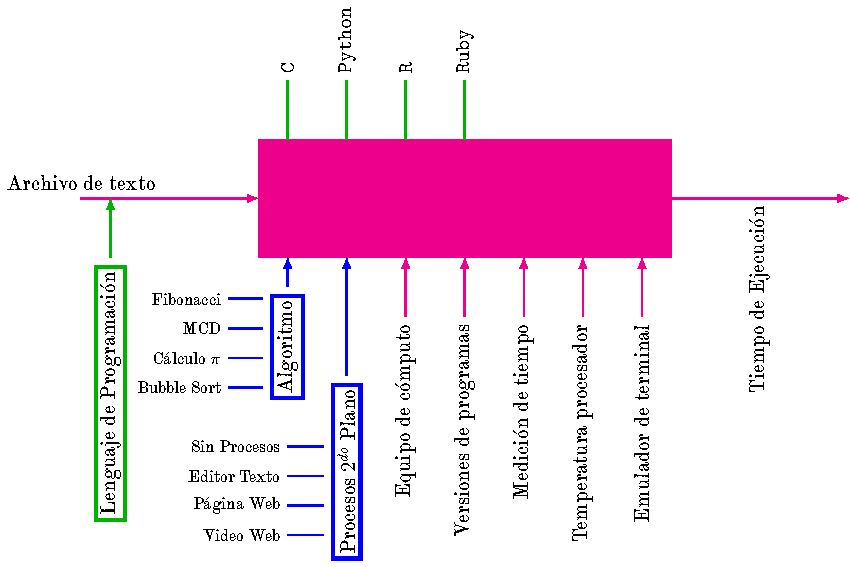
\includegraphics[width = 0.8\linewidth]{IMAGENES/2/tikz.pdf}
	\caption{Diagrama que representa el experimento propuesto.}
	\label{fig:diagrama_dcl}
\end{figure}
Y se tiene la siguiente tabla del orden de factores bloque.
\begin{table}[hbt!]
	\centering
	\footnotesize 
	\begin{tabular}{r|*{4}{c}}
		& Sin Procesos &	Editor de Texto &	Navegador en Pág. Web & Navegador Video Web. \\ \hline
		Fibinacci &  &   &   & \\
		MCD &  &   &  &  \\
		Cálculo de \(\pi\) &  &  &   &  \\
		Bubble Sort & &   &   & 
	\end{tabular}
	\caption{Diseño de Bloques DCL.} 
	\label{tab:diseño_dcl_exp}
\end{table}
% )))

\section{FACTORES DE RUIDO.} % (((
\label{sec:factores_ruido}

\subsection{--- Ordenador de Ejecución ---} % (((
\label{sub:condiciones}
\begin{minipage}{0.5\linewidth}
	\subsubsection{Hardware.} % (((
	\label{subs:hardware}
	\ttfamily
	\fbox{Modelo} Dell Inspiron 11 3000 11-3147. \\[2mm]
	\fbox{Procesador} Intel\textregistered Pentium(R) CPU N3540 @ 2.16GHz × 4 (Quad-core). \\[2mm]
	\fbox{Memoria RAM} \(\sim\)4GB of 1333 MHz DDR3L. \\[2mm]
	\fbox{Memoria} 500GB 5400 rpm 2.5" SATA II Hard Drive. \\[2mm]
	\fbox{Tarjeta Gráfica} Intel Atom Processor Z36xxx/Z37xxx Series Graphics \& Display. \\[2mm]
	\normalfont
	\addfontfeature{LetterSpace=-5}
	El resto de características físicas del equipo de cómputo pueden encontrarse en \micita{pag_web} y \micita{dell}.
	% )))
\end{minipage}\hspace{5mm}
\begin{minipage}{0.5\linewidth}
	\subsubsection{Software.} % (((
	\label{subs:software}
	\ttfamily
	\fbox{Sistema Operativo} (GNU/Linux) Ubuntu 20.04.4 LTS.\\[2mm]
	\fbox{Arquitectura} 64bits.\\[2mm]
	\fbox{Kernel} 5.13.0-40-generic.\\[2mm]
	\fbox{Shell} Bash 5.0.17.\\[2mm]
	\fbox{Emulador de Terminal} Kitty 0.22.2.\\[2mm]
	\normalfont
	\addfontfeature{LetterSpace=-5}
	El equipo de cómputo tenía \texttt{44min} encendido al realizar la primer prueba y las subsecuentes, como lo indica la Figura \ref{fig:caract}.
	Los procesos por defecto del sistema operativo son enunciados en la sección \ref{sub:segundo_plano}.
	% )))
\end{minipage}
\newpage
\begin{figure}[hbt!]
	\centering
	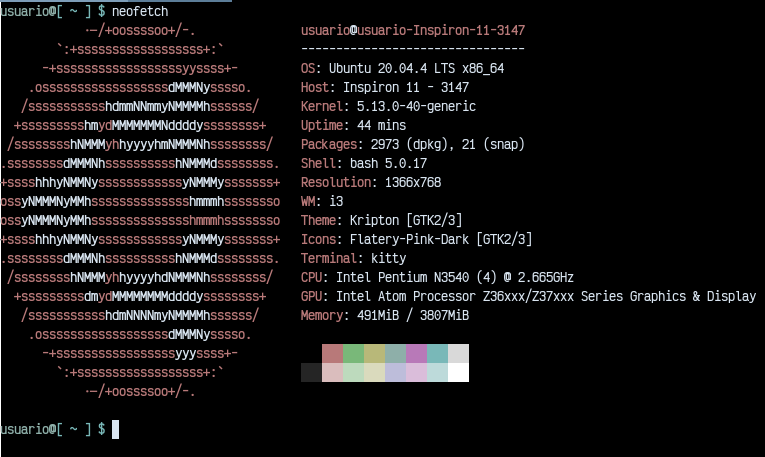
\includegraphics[width= 0.8 \linewidth]{IMAGENES/1/caracteristicas_equipo.png}
	\caption{Captura de pantalla de las características del equipo.}
	\label{fig:caract}
\end{figure}
% )))

\subsection{--- Medición del Tiempo ---} % (((
\label{sub:medicion_tiempo}
Para el registro de tiempos de ejecución, se hará uso del comando \codigo{time}, del sistema operativo Ubuntu en la versión \texttt{1.7} (así como se puede comprobar en la Figura \ref{fig:time}), cuya documentación se encuentra en \micita{manpage_time}.
\begin{figure}[hbt!]
	\centering
	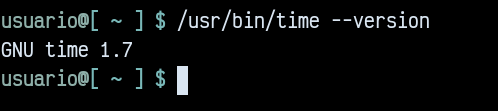
\includegraphics[width= 0.4 \linewidth]{IMAGENES/3/time.png}
	\caption{Captura de pantalla desde la línea de comandos para ver la version del comando \codigo{time}.}
	\label{fig:time}
\end{figure}\\
En cada proceso ejecutado por el sistema operativo, hay 3 eventos importantes del procesador que pueden medirse (en el tiempo) con el programa \codigo{time}.
\begin{enumerate}[noitemsep]
	\item \texttt{[Real Time]} Es la diferencia de registros obtenidos del reloj interno integrado del sistema operativo. El primer registro se realiza al empezar el proceso en terminal. El segundo registro se realiza cuando el proceso ha finalizado dentro del emulador de terminal, incluyendo así, el tiempo de posibles Input\(/\)Output desplegados por el programa.
	\item \texttt{[User Time]} Cantidad de tiempo en que el \texttt{CPU} usa en el modo usuario en el proceso.
		También se le conoce como modo \texttt{no-privilegiado}.
		En este modo, ciertas funciones no están disponibles por condiciones de hardware.
	\item \texttt{[System Time]} Cantidad de tiempo en que el \texttt{CPU} usa dentro del kernel del sistema operativo para ejecutar un proceso del programa.
		También se conoce como modo \texttt{privilegiado}.
		En este modo, se puede realizar cualquier instrucción que la arquitectura del sistema operativo permita. Sin embargo, no siempre es necesario acceder a éste modo.
\end{enumerate}
Consulte \micita{explicacion_time} y \micita{wiki_modos}. \\[2mm]
Se centrará la atención del expeirmento únicamente para medir el tiempo Real, es decir, el que experimentará el usuario final con su programa, debido a que se desea medir el impacto del lenguaje de programación en el segundo sector demográfico descrito en la sección \ref{sub:motivacion}.
\newpage
Se despliega un ejemplo del comando en a Figura \ref{fig:incert}, para observar que la incertidumbre de medición es de \(\pm 0.5\) milisegundos.
\begin{figure}[hbt!]
	\centering
	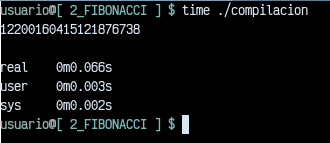
\includegraphics[width= 0.4 \linewidth]{IMAGENES/3/incertidumbre.png}
	\caption{Ejemplo de ejecución del comando \codigo{time}, midiendo una compilación en el lenguaje \texttt{C}.}
	\label{fig:incert}
\end{figure}
% )))

% )))

\section{ALEATORIZACIÓN.} % (((
\label{sec:aleatorizacion}
Como se indicó en la sección \ref{subs:definicion_de}, se requiere tener una elección aleatoria sobre el orden de las corridas experimentales.
Dado que, sólo se tendrá un factor controlable por cada una de las configuraciones de los bloques, entonces se asignarán los factores controlables aleatoriamente a cada celda de la matriz de la tabla de Diseño Cuadro Latino. \\[2mm]

Se hace uso del programa escrito en \micita{rosseta_rls} (adaptado en el archivo \codigo{GENERACION\textunderscore DISENO.c}, en % referencia github
% TODO: REFERENCIA A REPOSITORIO.
), y se ejecuta con la siguiente instrucción de \codigo{Bash}.
\begin{lstlisting}
g++ GENERACION_DISENO.c -o ./compilacion && ./compilacion > output.txt
\end{lstlisting}
Y se tiene el siguiente resultado
\begin{lstlisting}[backgroundcolor=\color{gray!15}]
[Ruby, Python, R, C]
[R, Ruby, C, Python]
[Python, C, Ruby, R]
[C, R, Python, Ruby]
\end{lstlisting}
Así, se escribe el diseño en la Tabla \ref{tab:diseño_dcl_exp}, y se coloca en la base de datos del repositorio
% TODO: ESCRIBIR REFERENCIA A REPOSITORIO.
\begin{table}[hbt!]
	\centering
	\footnotesize 
	\begin{tabular}{|r|*{4}{c|}}
		\hline 
		& Fibinacci &	MCD &	Cálculo de \(\pi\) & Bubble Sort \\ \hline
		Sin procesos & Ruby &  Python &  R &  C\\
		Editor de Texto & R &  Ruby &  C &  Python\\
		Navegador en Pág. Web & Python &  C &  Ruby &  R\\
		Navegador en Video Web & C &  R &  Python &  Ruby \\ \hline
	\end{tabular}
	\caption{Aleatorizaión del diseño.} 
	\label{tab:experimento_completo}
\end{table}\\
Se tiene un DCL no--estándar.
% )))

\section{NIVELES DE FACTOR CONTROLABLE.} % (((
\label{sec:niveles_fact_control}
Se escriben las versiones a ejecutar de los lenguajes de programación del DCL de la sección \ref{sec:adaptacion_exp}.
\begin{enumerate}[noitemsep]
	\item[\fbox{\texttt{C}}] El programa en el sistema operativo es \codigo{g++ 9.4.0}.
	\item[\fbox{\texttt{Python}}] \codigo{Python 3.8.10}.
	\item[\fbox{\texttt{R}}] \codigo{Rscript front-end version 4.1.2 (2021-11-01) -- "Bird Hippie" x86\textunderscore 64-pc-linux-gnu}.
	\item[\fbox{\texttt{Ruby}}] \codigo{ruby 2.7.0p0 (2019-12-25 revision 647ee6f091) [x86\textunderscore 64-linux-gnu]}
\end{enumerate}
% )))

\section{CONFIGURACIÓN DE BLOQUES.} % (((
\label{sec:conf_bloques}

\subsection{--- Algoritmos Seleccionados para Test de Rapidez ---} % (((
\label{sub:algoritmos}
% TODO: PONER REPOSITORIO.
Se esbozan los \(4\) algoritmos utilizados en el diseño experimental, cuyos archivos están licenciados con GPLv3, y pueden encontrarse en el repositorio % link
Estos algoritmos fueron escritos en cada lenguaje usando su documentación básica. 
 
\subsubsection{Números de Fibonacci.} % (((
\label{subs:fibo}
\fbox{
	\ttfamily
% \begin{minipage}{0.45\linewidth}
	\begin{algorithm}[H]
		\SetAlgoLined
		\SetKwProg{Fn}{Funcion}{ is}{end}
		\SetKwFunction{Fibo}{Fibonacci}
		\Fn{\Fibo(\(n\))}{
		\KwData{f\textunderscore actual = 0, f\textunderscore siguiente  = 1, aux = 0}
		\For{\(i \leqslant n\)}{
			aux = f\textunderscore actual + f\textunderscore siguiente\;
			f\textunderscore actual = f\textunderscore siguiente\;
			f\textunderscore siguiente = aux \tcc*[r]{orden de \(O(1)\)}
		}
		}
		Imprimir Fibonacci(46)\;
	\end{algorithm}
% \end{minipage}
}
Este algoritmo es de orden \(O(n)\), donde \(n\) es el número requerido.
% Está inspirado del repositorio de .
% )))

\subsubsection{Máximo Común Divisor.} % (((
\label{subs:mcd}
\fbox{
	\ttfamily
	\begin{algorithm}[H]
		\SetAlgoLined
		\SetKwProg{Fn}{Function}{ is}{end}
		\SetKwFunction{MCD}{Max\_Com\_Div}
		\Fn{\MCD (primer\_num , segundo\_num)}{
			residuo = mod(primer\_num,segundo\_num)\;
			\While{residuo \(\ne 0\)}{
				primer\_num = segundo\_num\;
				segundo\_num  = residuo\;
				residuo = mod(primer\_num,segundo\_num) \tcc*[r]{orden de \(O(\log n)\)}
			}
		}
		\MCD(6983776800,5587021440)\;
	\end{algorithm}
}
Este algoritmo es de orden \(O(n \log n)\), puesto que depende de lo largo que sea el número se efectuará el algoritmo de Euclides \codigo{mod} que es de complejidad \(O(\log n)\).
% Está inspirado del repositorio de .
% )))

\subsubsection{Cálculo de Pi.} % (((
\label{subs:calc_pi}
\fbox{
	\ttfamily
	\begin{algorithm}[H]
		\SetAlgoLined
		\SetKwProg{Fn}{Function}{ is}{end}
		\SetKwFunction{pi}{Aprox\_Pi}
		\KwData{\(a = 0\) , \(b = 1\) , \(n = 100,000\)}
		suma  = 0\;
		h = (b-a) /n\;
		\For{\(i \leqslant n\)}{
			suma = suma + sqrt(1 - (a+i*h) * (a+i*h)) \tcc*[r]{orden de \(O(2^n)\)}
		}
		suma = h * [(b-a)/2 + suma]\;
		Imprimir suma\;
	\end{algorithm}
}
Este algoritmo es de orden \(O(n 2^n)\), puesto que la función \codigo{sqrt()} es de orden \(O(2^n)\).
% Está inspirado del repositorio de .
% )))

\subsubsection{Bubble Sort.} % (((
\label{subs:bubble_sort}
\fbox{
	\ttfamily
	\begin{algorithm}[H]
		\SetAlgoLined
		\SetKwProg{Fn}{Function}{ is}{end}
		\SetKwFunction{ord}{Ordenamiento Burbuja}
		\KwData{a = [564, 550, 34, \(\;\ldots,\;\) 165]}\;
		\Fn{\ord(a)}{
			\For{\(j \leqslant\) length(\(a\))}{
				\For{\(i \leqslant j\)}{
					\If{\(a[i] < a[j]\)}{
						aux = a[i]\;
						a[i] = a[i+1]\;
						a[i+1] = aux \tcc*[r]{orden de \(O(1)\)}
					}
				}
			}
			return a\;
		}
	\end{algorithm}
}
Este algoritmo es de orden \(O(n^2)\), por los dos procesos \codigo{For}.
La cadena inicial \codigo{a} tiene los \(1,000\) números naturales desordenados, y fue generada en python.
Vease el código fuente en [] para la revisión de la cadena introducida.
% Está inspirado del repositorio de .
% )))

% )))

\subsection{--- Procesos en Segundo Plano ---} % (((
\label{sub:segundo_plano}
\begin{enumerate}
	\item[\fbox{Sin procesos}] Se tiene sólo la ejecución del programa más los procesos necesarios para que el sistema operativo funcione (en la Figura \ref{fig:sin_procesos}), junto con la terminal donde se ejecutan los scripts de la sección \ref{sub:algoritmos}. Pueden consultarse los procesos activos detalladamente en []
% TODO: referenciar repositorio github.
		\begin{figure}[hbt!]
			\centering
			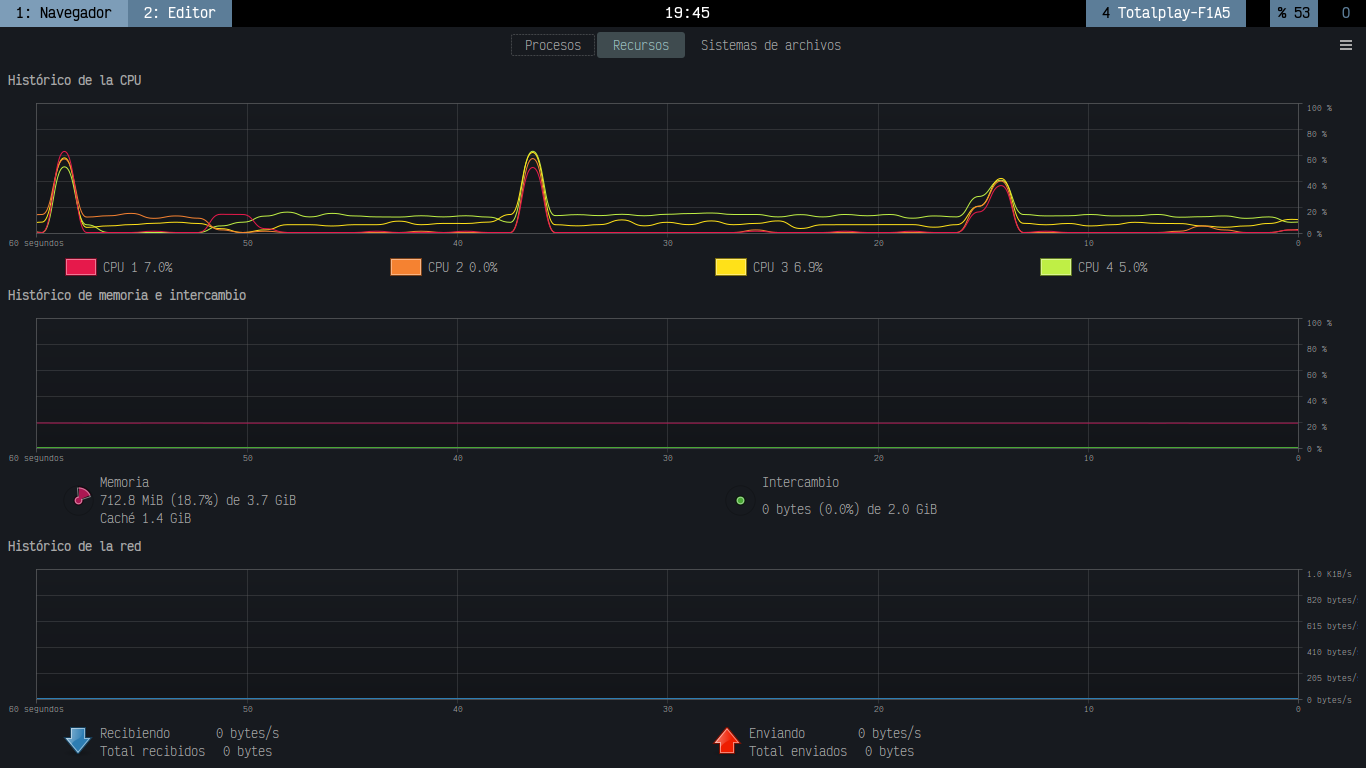
\includegraphics[width= 0.9 \linewidth]{IMAGENES/6/1_sin_procesos}
			\caption{Procesadores trabajando únicamente con los procesos por defecto del SO.}
			\label{fig:sin_procesos}
		\end{figure}
		\newpage
	\item[\fbox{Editor de Texto}] Se elige SublimeText (TM), por ser uno de los editores de texto más utilizados en ordenadores con relativos bajos resursos (consulte \micita{editors}). Los procesadores prsentaron el comportamiento de la Figura \ref{fig:subl} (nuevamente, las capturas de pantalla de todos los procesos se encuentra en).
		\begin{figure}[hbt!]
			\centering
			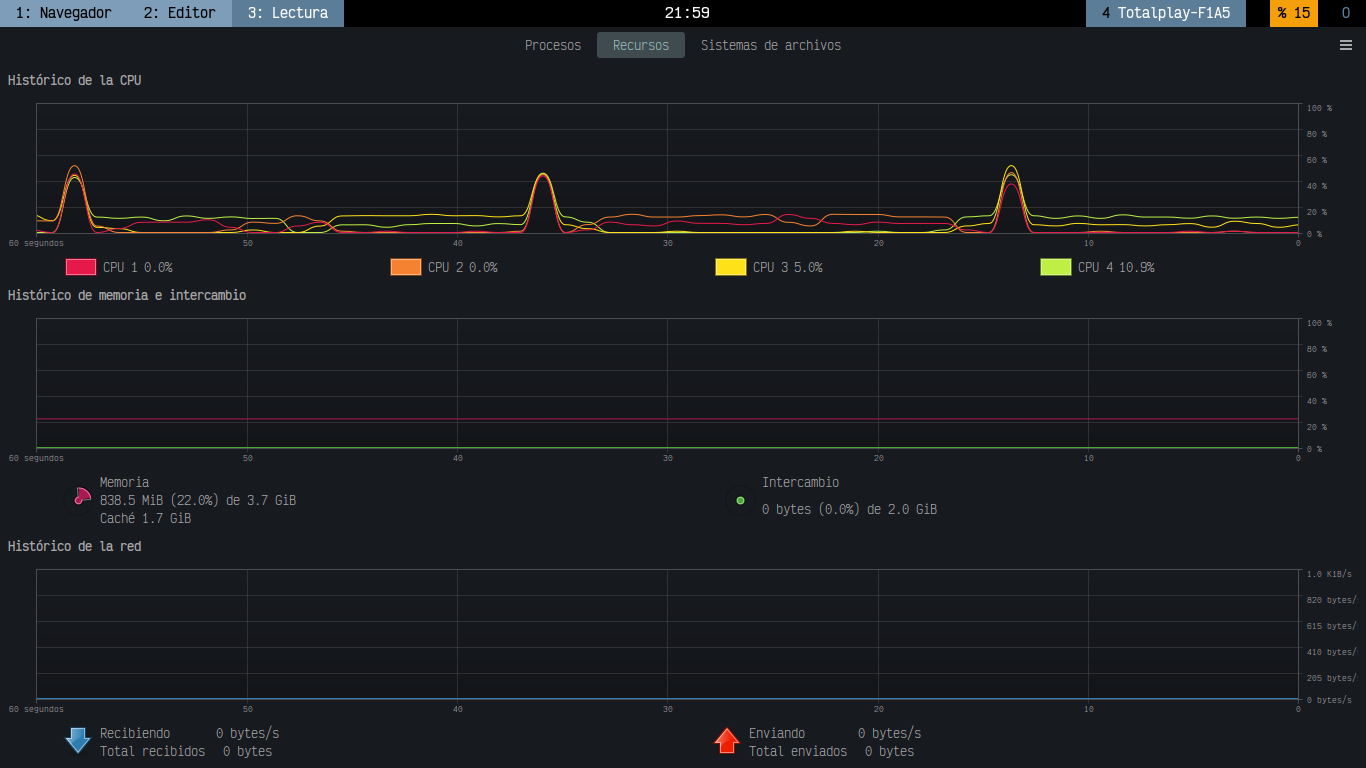
\includegraphics[width= 0.8 \linewidth]{IMAGENES/6/4_sublime_text}
			\caption{Procesadores trabajando con Sublime Text.}
			\label{fig:subl}
		\end{figure}
	\item[\fbox{Página Web}] El ordenador de ejecución tenía las siguientes características en la ejecución de Firefox con la página de internet \texttt{https://www.office.com/} abierta.
		\begin{figure}[hbt!]
			\centering
			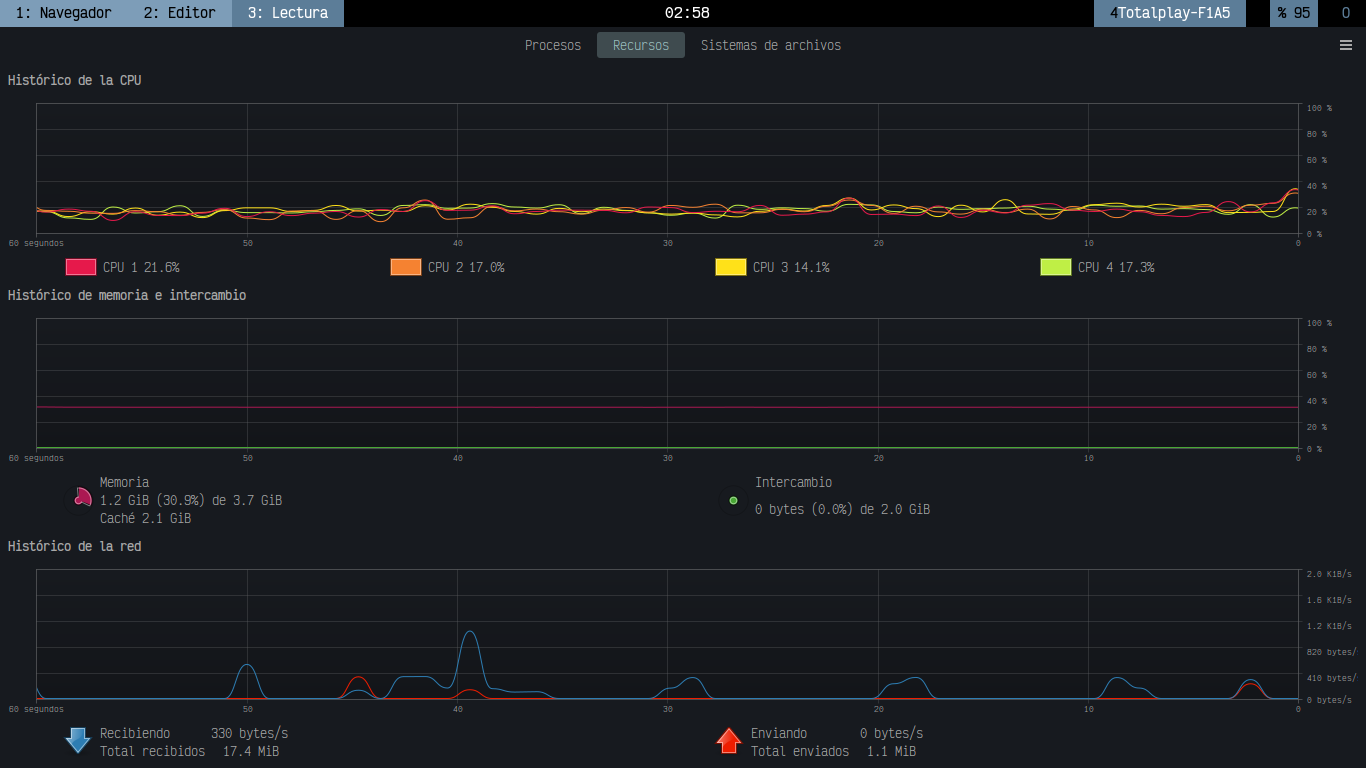
\includegraphics[width= 0.8 \linewidth]{IMAGENES/6/6_firefox_web}
			\caption{Procesadores con el navegador abierto en la página descrita.}
			\label{fig:firefox_1}
		\end{figure}
	\item[\fbox{Video Web}] Se elige la plataforma de Youtube en el video \texttt{https://www.youtube.com/watch?v=grBFMP3HDZA}.
		El cuál, en el ordenador de ejecución, tenía las siguientes características.
		\begin{figure}[hbt!]
			\centering
			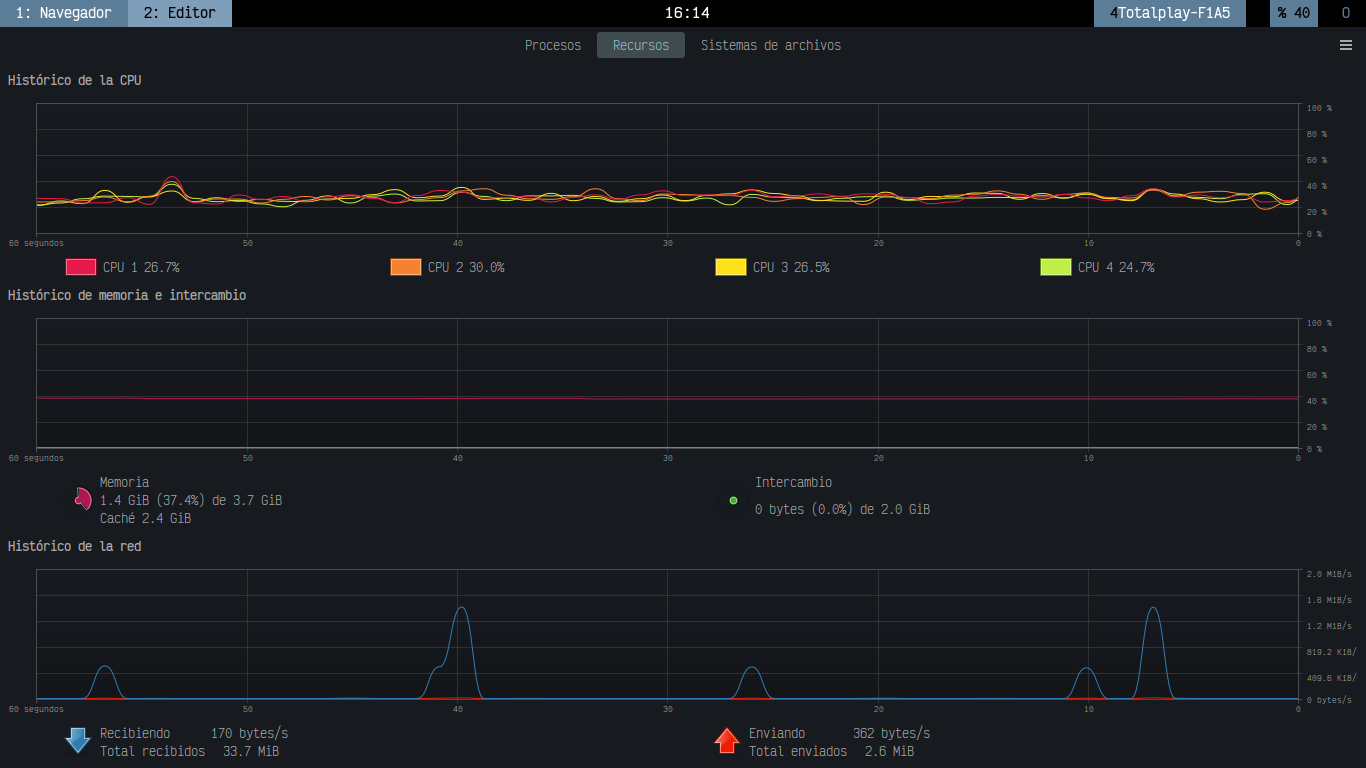
\includegraphics[width= 0.8 \linewidth]{IMAGENES/6/8_firefox_video}
			\caption{Procesadores ejecutando el video descrito en Firefox.}
			\label{fig:video}
		\end{figure}
\end{enumerate}
% )))

% )))

\section{METODOLOGÍA DEL EXPERIMENTO.} % (((
Como lo indica la Figura \ref{fig:caract}, el ordenador estuvo \(44min\) encendido al realizar la primer prueba de la Tabla \ref{tab:experimento_completo}.
Se realiza cada uno de los registros de tiempos de ejecución de forma aleatoria. \\[2mm]

Para minimizar el nivel de impresición del tiempo registrado computacionalmente, se realizan \(6\) repeticiones para cada una de las \(16\) mediciones, y se considerará como valor real su promedio aritmético.
Los datos completos pueden consultarse en % link.
% TODO: REFERENCIAR REPO.
A continuación se escriben los comandos utilizados en cada programa. \\[2mm]
\begin{minipage}{0.5\linewidth}
	\subsection{--- C ---} % (((
	\label{sub:lenguaje_c}
	Se realiza la compilación de cada archivo fuente \codigo{archivo.c}, mediante el programa \codigo{g++}.
	\begin{lstlisting}[language = bash]
g++ archivo.c -o ./compilacion
	\end{lstlisting}
	Dado que el experimento consiste en medir el tiempo que toma el archivo ejecutable \codigo{./compilacion} en completar la tarea deseada, se usa el programa \codigo{time}. Y se registra el tiempo generado por el siguiente comando.
	\begin{lstlisting}[language = bash]
time ./compilacion
	\end{lstlisting}
	El resto de lenguajes de programación no poseen archivos ejecutables.
	% )))
\end{minipage}\hspace{5mm}
\begin{minipage}{0.5\linewidth}

	\subsection{--- Python ---} % (((
	\label{sub:lenguaje_python}
	Se realiza el registro con el comando \codigo{time}, de la ejecución del programa \codigo{python3}.
	\begin{lstlisting}[language = bash]
time python3 archivo.py
	\end{lstlisting}
	% )))

	\subsection{--- R ---} % (((
	\label{sub:lenguaje_r}
	El comando que registra los tiempos de ejecución es el siguiente.
	\begin{lstlisting}[language = bash]
time Rscript archivo.r
	\end{lstlisting}
	% )))

	\subsection{--- Ruby ---} % (((
	\label{sub:lenguaje_ruby}
	Se registran los tiempos de medición con el siguiente comando.
	\begin{lstlisting}[language = bash]
time ruby archivo.rb
	\end{lstlisting}
	% )))

\end{minipage}

% )))

\newpage

\section{RESULTADOS.} % (((
\label{sec:resultados}
Se registra en la Tabla , los valores registrados con los promedios aritméticos de \(6\) tiempos de ejecución de cada programa en las condiciones de cada bloque.
La base de datos completa puede consultarse en 
% TODO. REFERENCIA REPOSITORIO GITHUB.
\begin{table}[hbt!]
	\centering
	\footnotesize 
	\begin{tabular}{|r|*{4}{l|}}
		\hline 
		& Sin Procesos &	Editor de Texto &	Navegador en Pág. Web & Navegador Video Web. \\ \hline
		Fibinacci & Ruby\((0.1878333)\) &  Python\((0.072)\) &  R\((0.631)\) &  C\((0.004166667)\)\\
		MCD & R\((0.6243333)\) &  Ruby\((0.1828333)\) &  C\((0.0055)\) &  Python\((0.6341667)\)\\
		Cálculo de \(\pi\) & Python\((1.1695)\) &  C\((0.015)\) &  Ruby\((0.2618333)\) &  R\((0.6631667)\)\\
		Bubble Sort & C\((0.01783333)\) &  R\((2.064333)\) &  Python\((0.4051667)\) &  Ruby\((0.35)\) \\ \hline
	\end{tabular}
	\caption{Aleatorizaión del diseño.} 
	\label{tab:resultados}
\end{table}
% )))

\section{ANÁLISIS ESTADÍSTICO.} % (((

Los resultados se evaluarán a un nivel de confianza del \(1- \alpha = 95\)\textsc{\%}, es decir, se toma \(\alpha = 0.05\).

\subsection{--- Diagrama de Cajas Simultáneas ---} % (((
\label{sub:cajas}
\begin{minipage}{0.65\linewidth}
	\includegraphics[width= 0.9 \linewidth, page = 1]{IMAGENES/9/RPlots.pdf}
\end{minipage}
\begin{minipage}{0.35\linewidth}
	Se concluye que
	\begin{enumerate}
		\item \texttt{Python}, \texttt{R} y \texttt{Ruby} presentan sesgo a la derecha.
		\item \texttt{R}  y \texttt{Ruby} comparten más del \(75\)\textsc{\%} de sus datos con \texttt{Python}.
		\item \texttt{Python} presenta una mayor variabilidad que el resto de lenguajes.
	\end{enumerate}
\end{minipage}
% )))

\subsection{--- Supuestos del Modelo de Regresión Lineal ---} % (((
\label{sub:supuestos_modelo}
\begin{table}[hbt!]
	\centering
	\begin{tabular}{|*{4}{l|}}
		\hline 
		Supuesto & Test & Valor--\(p\) & Conclusión \\ \hline
		Normalidad & Shapiro--Wilk & \(0.3323\) & Se cumple el supuesto de realidad \\ \hline
		Homocedasticidad & Levene & \(0.4367\) & Se cumple el supuesto de homocedasticidad \\ \hline
		Independencia & Durbin--Watson & \(0.6498\) & Se cumple el supuesto de independencia \\ \hline
	\end{tabular}
	\label{tab:supuestos}
\end{table}
% )))

\newpage

\subsection{--- ANOVA ---} % (((
\label{sub:anova}
Dada la verificación de los supuestos, se realiza la Tabla Anova (código y resultados en).
\begin{table}[hbt!]
	\footnotesize
	\centering
	\begin{tabular}{|*{6}{l|}}
		\hline
		F. Variabilidad                    & Grados de Libertad & Suma de Cuadrados & Cuadrados Medios & F & Valor--\(p\) \\ \hline
		F.Control(Lenguaje)                & 3 & 2.18778 & 0.72926  & 2.9085 & 0.1231 \\ \hline
		Bloque1(Algoritmo)                 & 3 & 0.52841 & 0.17614  & 0.7025 & 0.5843 \\ \hline
		Bloque2(Procesos \(2^{do}\) plano) & 3 & 0.14793 & 0.04931  & 0.1967 & 0.8950 \\ \hline
		Residuals                          & 6 & 1.50440 & 0.25073  &        &        \\ \hline
		Total                              &12 & 4.36852 &          &        & \\ \hline
	\end{tabular}
	\label{tab:anova}
\end{table}
Se observa que la columna \texttt{[Valor-p]} contiene los percentiles de las pruebas de hipótesis (1), (2) y (3), respectivamente. Las cuales adaptadas al modelo estadístico son las siguientes.
\begin{enumerate}
	\item[\fbox{Hip. Principal}] Se re-escribe (1).
		\[
			\begin{array}{rl}
				H_0 \;:\; & \mbox{Todos los lenguajes de programación estudiados tienen el mismo tiempo de ejecución promedio.} \\
				H_a \;:\; & \mbox{Hay al menos un lenguaje analizado que tiene un tiempo promedio de ejecución diferente.}
			\end{array}
		\]
	\item[\fbox{Hip. Secundaria 1}] Se re-escribe (2).
		\[
			\begin{array}{rl}
				H_0 \;:\; & \mbox{El tiempo de ejecución promedio no es afectado por el algoritmo programado.} \\
				H_a \;:\; & \mbox{Hay al menos un algoritmo que produce un tiempo de ejecución promedio diferente.}
			\end{array}
		\]
		Se tiene que \textit{valor-p\(= 07025 > \alpha\)}, entonces no se rechaza \(H_0\) (es decir, el tiempo de ejecución promedio no es afectado por la complejidad algoritmica del programa).
		Se remueve ésta fuente de variabilidad y se realiza nuevamente el análisis en la sección \ref{sub:dbca}.
	\item[\fbox{Hip. Secundaria 2}] Se re-escribe (3).
		\[
			\begin{array}{rl}
				H_0 \;:\; & \mbox{El tiempo de ejecución promedio no es afectado por la cantidad de procesos en segundo plano.} \\
				H_a \;:\; & \mbox{Hay al menos un proceso en segundo plano que produce un tiempo de ejecución promedio diferente.}
			\end{array}
		\]
\end{enumerate}
% )))

\subsection{--- Reducción de Modelo a un DBCA ---} % (((
\label{sub:dbca}
Se redujo el modelo a la siguiente formulación de la ecuación (\ref{eq:modelo}) \(Y_{jh} = \mu + \tau _{h_{j}} + \delta _j + \varepsilon _{ij(h_{ij})}\), que es un DBCA. Y por tanto, se construye de nuevo la Tabla ANOVA.
\begin{table}[hbt!]
	\centering
	\footnotesize
	\begin{tabular}{|*{6}{l|}}
		\hline
		F. Variabilidad                   & Grados de Libertad & Suma de Cuadrados & Cuadrados Medios & F & Valor--\(p\) \\ \hline
		F.Control(Lenguaje) & 3 & 2.18778 & 0.72926  & 3.9722 & 0.04677\\ \hline
		Bloque2(Procesos \(2^{do}\) Plano)  & 3 & 0.14793 & 0.04931  & 0.2183 & 0.88126\\ \hline
		Residuals           & 9 & 2.03281 & 0.22587  &        &        \\ \hline
		Total               &12 & 4.36852 &          &        & \\ \hline
	\end{tabular}
	\label{tab:nuevo_modelo}
\end{table}
\begin{enumerate}
	\item[\fbox{Hip. Principal}] \color{white} c \color{black}
		\[
			\begin{array}{rl}
				H_0 \;:\; & \mbox{Todos los lenguajes de programación estudiados tienen el mismo tiempo de ejecución promedio.} \\
				H_a \;:\; & \mbox{Hay al menos un lenguaje analizado que tiene un tiempo promedio de ejecución diferente.}
			\end{array}
		\]
	\item[\fbox{Hip. Secundaria 2}] \color{white} c \color{black}
		\[
			\begin{array}{rl}
				H_0 \;:\; & \mbox{El tiempo de ejecución promedio no es afectado por la cantidad de procesos en segundo plano.} \\
				H_a \;:\; & \mbox{Hay al menos un proceso en segundo plano que produce un tiempo de ejecución promedio diferente.}
			\end{array}
		\]
		Se tiene que \(valor-p = 0.88126 > \alpha\), entonces no se rechaza \(H_0\).
		Por tanto, los procesos en segundo plano no afectan a los tiempos promedio de ejecución.
		Se reduce el modelo a un DCA en la sección \ref{sub:dca}.
\end{enumerate}
% )))

\subsection{--- Reducción a un DCA ---} % (((
\label{sub:dca}
Se construye la tabla ANOVA.
\begin{table}[hbt!]
	\centering
	\footnotesize
	\begin{tabular}{|*{6}{l|}}
		\hline
		F. Variabilidad     & Grados de Libertad & Suma de Cuadrados & Cuadrados Medios & F & Valor--\(p\) \\ \hline
		F.Control(Lenguaje) &  3 & 2.1878 & 0.72926  & 4.0129 & 0.03428\\ \hline
		Residuals           & 12 & 2.1807 & 0.18173  &        &        \\ \hline
		Total               &12 & 4.36852 &          &        & \\ \hline
	\end{tabular}
	\label{tab:nuevo_modelo}
\end{table}
Finalmente, se contesta la Hipótesis Principal.
\begin{enumerate}
	\item[\fbox{Hip. Principal}] \color{white} c \color{black}
		\[
			\begin{array}{rl}
				H_0 \;:\; & \mbox{Todos los lenguajes de programación estudiados tienen el mismo tiempo de ejecución promedio.} \\
				H_a \;:\; & \mbox{Hay al menos un lenguaje analizado que tiene un tiempo promedio de ejecución diferente.}
			\end{array}
		\]
		Y en este caso tenemos que \(valor-p = 0.03 < \alpha\), por lo que se rechaza \(H_0\).
		Así, existe un lenguaje de programación que tiene un tiempo de ejecución promedio diferente al resto.
		Se observará cuál es diferente en la sección .
\end{enumerate}
% )))

\subsection{--- Tratamientos Diferentes ---} % (((
\label{sub:trata_diferentes}
Se ejecuta LSD (véase el repositorio), y se observa lo siguiente.
% TODO: AÑADIR EL REPOSITORIO.
       % Respuesta         std r         LCL       UCL         Min        Max
% C      0.0106250 0.006808728 4 -0.60199990 0.6232499 0.004166667 0.01783333
% Python 0.5702084 0.461407795 4 -0.04241655 1.1828333 0.072000000 1.16950000
% R      0.9957082 0.712618224 4  0.38308335 1.6083332 0.624333300 2.06433300
% Ruby   0.2456250 0.078399676 4 -0.36699993 0.8582499 0.182833300 0.35000000
% 
% Alpha: 0.05 ; DF Error: 6
% Critical Value of t: 2.446912 
% 
% least Significant Difference: 0.8663824 
% 
% Treatments with the same letter are not significantly different.
% 
\begin{lstlisting}[language = R]
       Respuesta groups
R      0.9957082      a
Python 0.5702084     ab
Ruby   0.2456250     ab
C      0.0106250      b
\end{lstlisting}
% )))

% )))

\section{CONCLUSIONES.} % (((
% (ojalá) que C sea más rapido que todos.
% matlab es el más lento de todos.
% a pesar de que octave fue más lento en el cálculo de pi, al colocar el formato \texttt{[format long]} pudo establecer con una precisión de 10 digitos correctos de pi. (consúltese el repositorio).
% CONCLUSIÓN ESTADÍSTICA DEL EXPERIMENTO.
% )))

\section{FUTURA INVESTIGACIÓN.} % (((
un diseño que permita considerar todos los lenguajes en las mismas condiciones (la misma configuración de bloques), esto es, aplicar un DCA en cada una de las posibles configuraciones de los 2 Bloques.
% incluir programas y procesos algoritmicos que requieran aleatorización 
% i.e. la construcción de números pseudoaleatorios por parte del lenguaje.
% )))

% TODO: CREAR REPOSITORIO EN GITHUB. incluir licencia GPLv3

\newpage

% === REFERENCIAS === (((
\bibliography{Referencias}
\bibliographystyle{unsrt}
% )))

\end{document}
